\documentclass{article} % For LaTeX2e
\usepackage{CJK}
\usepackage{project,times}
\usepackage{hyperref}
\usepackage{url}
\usepackage{graphicx}
\usepackage{caption}
\usepackage{subfig}
\usepackage{bm}
\usepackage{mathrsfs}
\usepackage{bbm}
\usepackage{amsmath,amsthm,amsfonts,amssymb,amscd}
\usepackage{booktabs}
%\documentstyle[nips12submit_09,times,art10]{article} % For LaTeX 2.09

\newcommand{\beq}{\vspace{0mm}\begin{equation}}
\newcommand{\eeq}{\vspace{0mm}\end{equation}}
\newcommand{\beqs}{\vspace{0mm}\begin{eqnarray}}
\newcommand{\eeqs}{\vspace{0mm}\end{eqnarray}}
\newcommand{\barr}{\begin{array}}
\newcommand{\earr}{\end{array}}
\newcommand{\Amat}[0]{{{\bf A}}}
\newcommand{\Bmat}{{\bf B}}
\newcommand{\Cmat}{{\bf C}}
\newcommand{\Dmat}{{\bf D}}
\newcommand{\Emat}[0]{{{\bf E}}}
\newcommand{\Fmat}[0]{{{\bf F}}\xspace}
\newcommand{\Gmat}{{\bf G}}
\newcommand{\Hmat}{{\bf H}}
\newcommand{\Imat}{{\bf I}}
\newcommand{\Jmat}[0]{{{\bf J}}\xspace}
\newcommand{\Kmat}[0]{{{\bf K}}\xspace}
\newcommand{\Lmat}[0]{{{\bf L}}}
%\newcommand{\Mmat}[0]{{{\bf M}}\xspace}
\newcommand{\Mmat}{{\bf M}}
\newcommand{\Nmat}[0]{{{\bf N}}\xspace}
\newcommand{\Omat}[0]{{{\bf O}}}
\newcommand{\Pmat}{{\bf P}}
\newcommand{\Qmat}[0]{{{\bf Q}}\xspace}
\newcommand{\Rmat}[0]{{{\bf R}}}
\newcommand{\Smat}[0]{{{\bf S}}}
\newcommand{\Tmat}[0]{{{\bf T}}}
\newcommand{\Umat}[0]{{{\bf U}}}
\newcommand{\Vmat}[0]{{{\bf V}}}
\newcommand{\Wmat}[0]{{{\bf W}}}
\newcommand{\Xmat}[0]{{{\bf X}}}
\newcommand{\Ymat}{{\bf Y}}
%\newcommand{\Ymat}[0]{{{\bf Z}}}
\newcommand{\Zmat}{{\bf Z}}

\newcommand{\av}[0]{{\boldsymbol{a}}}
\newcommand{\bv}[0]{{\boldsymbol{b}}}
\newcommand{\cv}[0]{{\boldsymbol{c}}}
\newcommand{\dv}{\boldsymbol{d}}
\newcommand{\ev}[0]{{\boldsymbol{e}}\xspace}
\newcommand{\fv}[0]{{\boldsymbol{f}}\xspace}
\newcommand{\gv}[0]{{\boldsymbol{g}}\xspace}
\newcommand{\hv}[0]{{\boldsymbol{h}}}
\newcommand{\iv}[0]{{\boldsymbol{i}}\xspace}
\newcommand{\jv}[0]{{\boldsymbol{j}}\xspace}
\newcommand{\kv}[0]{{\boldsymbol{k}}\xspace}
\newcommand{\lv}[0]{{\boldsymbol{l}}}
\newcommand{\mv}[0]{{\boldsymbol{m}}}
\newcommand{\nv}[0]{{\boldsymbol{n}}\xspace}
\newcommand{\ov}[0]{{\boldsymbol{o}}\xspace}
\newcommand{\pv}[0]{{\boldsymbol{p}}}
\newcommand{\qv}[0]{{\boldsymbol{q}}\xspace}
\newcommand{\rv}{\boldsymbol{r}}
\newcommand{\sv}[0]{{\boldsymbol{s}}}
\newcommand{\tv}[0]{{\boldsymbol{t}}\xspace}
\newcommand{\uv}{\boldsymbol{u}}
\newcommand{\vv}{\boldsymbol{v}}
\newcommand{\wv}{\boldsymbol{w}}
\newcommand{\xv}{\boldsymbol{x}}
\newcommand{\yv}{\boldsymbol{y}}
\newcommand{\zv}{\boldsymbol{z}}
\newcommand{\cdotv}{\boldsymbol{\cdot}}

\newcommand{\Gammamat}[0]{{\boldsymbol{\Gamma}}\xspace}
\newcommand{\Deltamat}[0]{{\boldsymbol{\Delta}}\xspace}
\newcommand{\Thetamat}{\boldsymbol{\Theta}}
\newcommand{\Betamat}{\boldsymbol{\Beta}}
\newcommand{\Lambdamat}{\boldsymbol{\Lambda}}
\newcommand{\Ximat}[0]{{\boldsymbol{\Xi}}\xspace}
\newcommand{\Pimat}[0]{{\boldsymbol{\Pi}}\xspace}
\newcommand{\Sigmamat}[0]{{\boldsymbol{\Sigma}}}
\newcommand{\Upsilonmat}[0]{{\boldsymbol{\Upsilon}}\xspace}
\newcommand{\Phimat}{\boldsymbol{\Phi}}
\newcommand{\Psimat}{\boldsymbol{\Psi}}
\newcommand{\Omegamat}[0]{{\boldsymbol{\Omega}}}

\newcommand{\alphav}{\boldsymbol{\alpha}}
\newcommand{\betav}[0]{{\boldsymbol{\beta}}}
\newcommand{\gammav}[0]{{\boldsymbol{\gamma}}\xspace}
\newcommand{\deltav}[0]{{\boldsymbol{\delta}}\xspace}
\newcommand{\epsilonv}{\boldsymbol{\epsilon}}
\newcommand{\zetav}[0]{{\boldsymbol{\zeta}}\xspace}
\newcommand{\etav}[0]{{\boldsymbol{\eta}}\xspace}
\newcommand{\ellv}[0]{{\boldsymbol{\ell}}}
\newcommand{\thetav}{\boldsymbol{\theta}}
\newcommand{\iotav}[0]{{\boldsymbol{\iota}}}
\newcommand{\kappav}[0]{{\boldsymbol{\kappa}}\xspace}
\newcommand{\lambdav}[0]{{\boldsymbol{\lambda}}}
\newcommand{\muv}[0]{{\boldsymbol{\mu}}}
\newcommand{\nuv}[0]{{\boldsymbol{\nu}}}
\newcommand{\xiv}[0]{{\boldsymbol{\xi}}}
\newcommand{\omicronv}[0]{{\boldsymbol{\omicron}}\xspace}
\newcommand{\piv}{\boldsymbol{\pi}}
\newcommand{\rhov}[0]{{\boldsymbol{\rho}}\xspace}
\newcommand{\sigmav}[0]{{\boldsymbol{\sigma}}\xspace}
\newcommand{\tauv}[0]{{\boldsymbol{\tau}}\xspace}
\newcommand{\upsilonv}[0]{{\boldsymbol{\upsilon}}\xspace}
\newcommand{\phiv}{\boldsymbol{\phi}}
\newcommand{\chiv}[0]{{\boldsymbol{\chi}}\xspace}
\newcommand{\psiv}{\boldsymbol{\psi}}
\newcommand{\varthetav}{\boldsymbol{\vartheta}}
\newcommand{\omegav}[0]{{\boldsymbol{\omega}}}
\newcommand{\R}{\mathbb{R}}
\newcommand{\E}{\mathbb{E}}

\newcommand{\Xcal}{\mathcal{X}}
\newcommand{\Ycal}{\mathcal{Y}}
\newcommand{\NNcal}{\mathcal{N}}
\newcommand{\Lcal}{\mathcal{L}}
\newcommand{\Ncal}{\mathcal{N}}
\newcommand{\Bcal}{\mathcal{B}}
\newcommand{\Dcal}{\mathcal{D}}
\newcommand{\Tcal}{\mathcal{T}}
\newcommand{\Pcal}{\mathcal{P}}
\newcommand{\Ical}{\mathcal{I}}
\newcommand{\Gcal}{\mathcal{G}}
\newcommand{\Scal}{\mathcal{S}}

\title{Convolutional Factor Analysis with Fast Gibbs Sampling Algorithms}

\author{
Zhe Gan(zg27) \\
Department of ECE, \ Duke University \\
\texttt{zhe.gan@duke.edu}
}

\newcommand{\fix}{\marginpar{FIX}}
\newcommand{\new}{\marginpar{NEW}}

\nipsfinalcopy

\begin{document}

\bibliographystyle{plain}
\maketitle

\begin{abstract}
This project aims to implement the convolutional factor-analysis model proposed in \cite{chen2011hierarchical}. The model parameters are learned within a Bayesian setting, employing Gibbs sampling, while the number of factors is inferred via the beta process. Preliminary experimental results on MNIST and Caltech 101 datasets demonstrate that the proposed model can achieve good performance.  
\end{abstract}

\section{Introduction}
%
There has been significant recent interest in multi-layered or ``deep'' models for representation of general data, with a particular focus on imagery. Popular deep learning models include: Deep Belief Network \cite{hinton2006fast}, Deep Boltzmann Machine \cite{salakhutdinov2009deep}, Convolutional Neural Networks \cite{lecun1998gradient} and Deconvolutional Networks \cite{zeiler2010deconvolutional}, etc. Among these, deep covolutional networks have demonstrated excellent performance on image classification tasks. There are at least two key components of this model: 1) convolution operator, which considers all possible shifts of canonical filters; 2) a deep architecture, in which the features of a given layer serve as the inputs to the next layer above. 

However, the training of a convolutional neural network is typically imposed as an optimization problem. In this course project, I will focus on developing Bayesian generative model for deep convolutional dictionary learning, based on the idea proposed in \cite{chen2011hierarchical}. As stated in the paper, some advantages of the proposed model are: (\emph{i}) the number of factors needed is inferred from the data by an Indian Buffet Process(IBP) \cite{griffiths2011indian} or Beta Process (BP) \cite{paisley2009nonparametric} construction; (\emph{ii}) fast computations are performed using Gibbs sampling, where the convolution operation is exploited directly within the update
equations; and (\emph{iii}) sparseness is imposed on the factor loadings and factor scores, via a Bayesian generalization of the L1 regularizer. 

Recently, I am focusing my research on designing efficient and scalable Bayesian inference algorithms for deep learning models. Therefore, the course project will be helpful for my research. 

\section{Model Formulation}
%
The proposed model is applicable to general data, for which a convolutional dictionary representation is appropriate. One may, for example, apply the model to one-dimensional signals such as audio, or to two-dimensional imagery. In this project, we focus on imagery, and hence assume two-dimensional signals and convolutions. 

Assume $N$ images $\{\Xmat_n\}_{n=1,\ldots,N}$, with $\Xmat_n \in R^{n_y \times n_x \times K_c}$, where $K_c$ is the number of color channels (\emph{e.g.}, for gray-scale images $K_c = 1$, while for RGB images $K_c = 3$); the images are analyzed jointly to learn the convolutional dictionary $\Dcal =\{\dv_k\}_{k=1,\ldots,K}$. In practice, the number of dictionary elements $K$ is made large, and we wish to infer the subset of $\Dcal$ that is actually needed to represent $\Xmat_n$. The dictionary elements are designed to capture local structure within $\Xmat_n$, and all possible two-dimensional (spatial) shifts of the dictionary elements are considered for representation of $\Xmat_n$. Specifically, consider the model
%
\begin{align}
\Xmat_n = \sum_{k=1}^K b_{nk} \Wmat_{nk} \ast \dv_{k}   + \epsilonv_{n},
\end{align}
%
where $\ast$ is the convolution operator, and $b_{nk} \in \{0,1\}$ indicates whether $\dv_k$ is used to represent $\Xmat_n$, and $\epsilonv_{n}$ represents the residual. Considering $\dv_k \in R^{n_y^{\prime} \times n_x^{\prime} \times K_c}$ (typically $n_x^{\prime} \ll n_x$ and $n_y^{\prime} \ll n_y$), the corresponding weights $ \Wmat_{nk}$ are of size $(n_y - n_y^{\prime}+1) \times (n_x - n_x^{\prime}+1)$, allowing for all possible shifts. We impose within the model that the $\{w_{nki}\}_{i\in \Scal}$ are sparse or nearly sparse, such that most $w_{nki}$ are sufficiently small to be discarded without significantly affecting the reconstruction of $\Xmat_n$, where the set $\Scal$ contains all possible indexes for dictionary shifts.

Within a Bayesian construction, the priors for the model may be represented as 
%
\begin{align}
b_{nk} &\sim \mbox{Bernoulli} (\pi_k), &  \pi_k &\sim \mbox{Beta} (1/K,b), \\
w_{nki} &\sim N (0,1/\alpha_{nki}), & \dv_k &\sim \prod_{j=1}^J \Ncal(0,1/\beta_j), & \epsilon_n &\sim \Ncal(0,\Imat_P \gamma_{n}^{-1}), \\
\alpha_{nki} &\sim \mbox{Ga} (e,f), & \gamma_n &\sim \mbox{Ga} (c,d), & \beta_j &\sim \mbox{Ga} (g,h)
\end{align}
%
where $J$ denotes the number of pixels in the dictionary elements $\dv_k$ and $d_{kj}$ is the $j$th component of $\dv_k$. $\mbox{Ga}(\cdot)$ denotes the gamma distribution. The integer $P$ denotes the number of pixels in $\Xmat_n$, and $\Imat_P$ represents a $P \times P$ identity matrix. $\{b,c,d,e,f,g,h\}$ are hyperparameters. In the limit $K \rightarrow \infty$, and upon marginalizing out $\{\pi_k\}_{k=1,\ldots,K}$, the above model corresponds to the IBP \cite{griffiths2005infinite} \cite{thibaux2007hierarchical}. While the model may look somewhat complicated, local conjugacy admits Gibbs sampling or variational Bayes inference.

\section{Inference}
%
The local conditional posterior distribution for all parameters of the model is manifested in closed form, yielding efficient Gibbs sampling algorithm. The FFT is leveraged to accelerate computation of the covolution operations.

For each MCMC iteration, the samples are drawn from the following conditional distributions:

\textbf{(1) For} $b_{nk}$ and $\Wmat_{nk}$ (\emph{i.e.} $\{w_{nki}\}_{i \in \Scal}$) : we have $p(b_{nk}=1|-) = \tilde{\pi}_{nk}$, and $p(w_{nki},i \in \Scal|-) = (1-b_{nk}) \Ncal(0,\alpha_{nki}^{-1}) + b_{nk} \Ncal (\mu_{nki},\Sigma_{nki})$, where $\Sigma_{nki} = (\dv_{ki}^\top \dv_{ki} \gamma_n + \alpha_{nki})^{-1}$, $\mu_{nki} = \Sigma_{nki} \gamma_n \Xmat_{nki}^\top \dv_{ki}$, with $\Xmat_{nki}= \Xmat_{-n} + b_{nk}\dv_{ki} w_{nki}$, and 
%
\begin{align}
\frac{\tilde{\pi}_{nk}}{1-\tilde{\pi}_{nk}} = \frac{\pi_k}{1-\pi_k} \cdot \frac{\Ncal (\Xmat_{nk}|\Wmat_{nk} \ast \dv_k, \gamma_n^{-1}\Imat_P)}{\Ncal (\Xmat_{nk}|0,\gamma_n^{-1}\Imat_P)}
\end{align}
%
Here $\Xmat_{nk}=\Xmat_{-n}+\Wmat_{nk} \ast \dv_k$, $\Xmat_{-n} = \Xmat_n - \sum_{k=1}^K b_{nk} \Wmat_{nk} \ast \dv_k$ and $b_{nk}$ is the most recent sample. Taking advantage of the convolution property, we simultaneously update the posterior mean and covariance of the coefficients for all the shifted versions of one dictionary element. Consequently, 
%
\begin{align}
\Sigmamat_{nk} &= 1 \oslash (\gamma_n ||\dv_k||_2^2 b_{nk} + \alphav_{nk}), \\
\muv_{nk} &= b_{nk} \gamma_n \Sigmamat_{nk} \odot (\Xmat_{-n} \ast \dv_k + ||\dv_k||_2^2 \Wmat_{nk})
\end{align}
%
where both of $\Sigmamat_{nk}$ and $\muv_{nk}$ have the same size with $\Wmat_{nk}$. The symbol $\odot$ is the element-wise product operator and $\oslash$ the element-wise division operator.

\textbf{(2) For} $\dv_k$: we have $p(d_{kj}|-) = \Ncal (\xi_{kj},\Lambda_{kj})$, where $\xi_{kj}$ and $\Lambda_{kj}$ is the $j$th element of the following vectors $\xiv_k$ and $\Lambdamat_k$, respectively.
%
\begin{align}
\Lambdamat_k &= 1 \oslash \left( \sum_{n=1}^N \gamma_n b_{nk} ||\Wmat_{nk}||_2^2 +\beta_k  \right), \\
\xiv_k &= \Lambdamat_k \odot \left( \sum_{n=1}^N b_{nk} \gamma_n (\Xmat_{-n} \ast \Wmat_{nk} + \dv_k ||\Wmat_{nk}||_2^2) \right)
\end{align} 

The remaining Gibbs updates are relatively standard, and are provided below. (\emph{i}) Sampling $\pi_k$: $p(\pi_k|-) = \mbox{Beta} (\tilde{a},\tilde{b})$, where $\tilde{a} = \sum_{n=1}^N b_{nk} + 1/K$, $\tilde{b} = N+b-\sum_{n=1}^N b_{nk}$; (\emph{ii}) Sampling $\gamma_n$: $p(\gamma_n|-) = \mbox{Ga} (\tilde{c},\tilde{d})$, where $\tilde{c} = c + 1/2$, $\tilde{d} = d + ||\Xmat_n||_2^2/2$; (\emph{iii}) Sampling $\alpha_{nki}$: $p(\alpha_{nki}|-) = \mbox{Ga} (\tilde{e},\tilde{f})$, where $\tilde{e} = e + 1/2$, $\tilde{f} = f + w_{nki}^2/2$; (\emph{iv}) Sampling $\beta_{kj}$: $p(\beta_{kj}|-) = \mbox{Ga} (\tilde{g},\tilde{h})$, where $\tilde{g} = g + 1/2$, $\tilde{h} = f + d_{kj}^2/2$.

During the inference, we perform efficient block Gibbs sampling by sampling each dictionary element and corresponding hidden units given other parameters fixed. Throughout the inference procedure, no matrix inversion is needed since the dictionary and hidden units (factor scores) have been factorized. In practice, we typically do not need a large number of iterations to achieve useful results (we focus on finding an MAP solution, rather than a full posterior). 

\section{Experiments}
%
We present the performance of the proposed model on a small subset of the two widely used datasets: MNIST and Caltech 101. In all experiments, we set $b=e=g=1$, $c=d=h=10^{-6}$, and $f=10^{-3}$. The truncation level of the number of factors are set to $36$. Since we only consider gray-scale images, and therefore $K_c = 1$. We collect $300$ samples, after first computing and discarding $200$ burn-in samples.

\begin{figure}
   \centering
   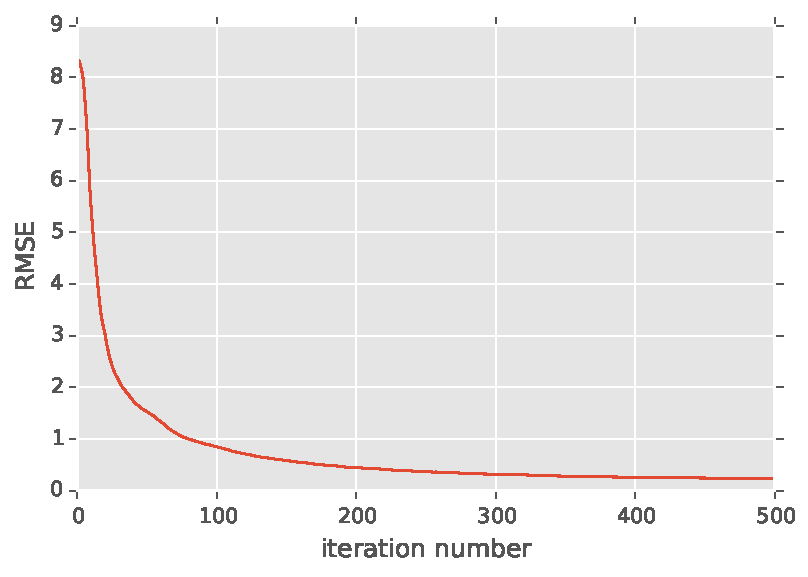
\includegraphics[width=6cm]{figures/mnist_mse}  
   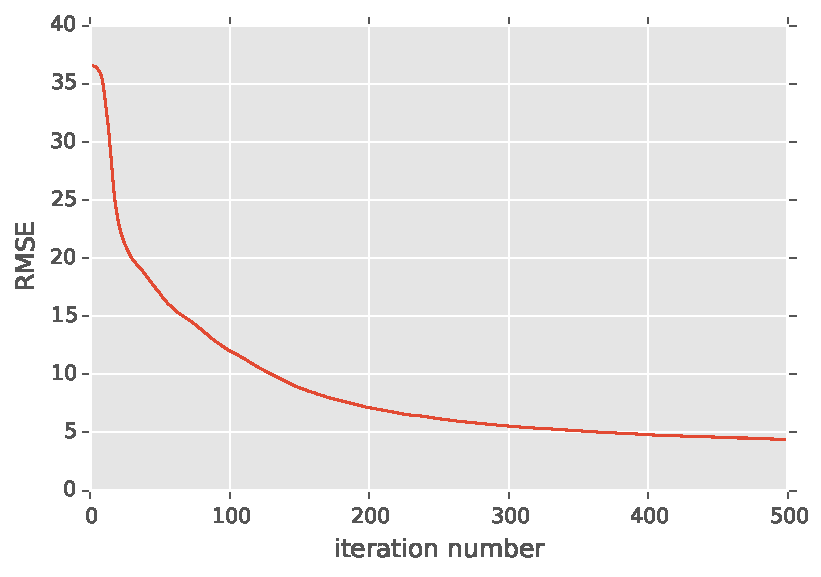
\includegraphics[width=6cm]{figures/face_mse} 
   \caption{\small{Root mean squared error as a function of iteration numbers. (Left) MNIST dataset. (Right) Caltech101 face dateset.}} \label{fig:mse}
\end{figure}

\subsection{MNIST Examples}

We first consider the widely studied MNIST dataset \footnote{http://yann.lecun.com/exdb/mnist/}, in which we perform analysis on 1000 images, each $28 \times 28$, for digits 0 through 9 (for each digit, we randomly select 10 images). The dictionary $\dv_k$ are of size $7 \times 7$.

\begin{figure}[h]
   \centering
   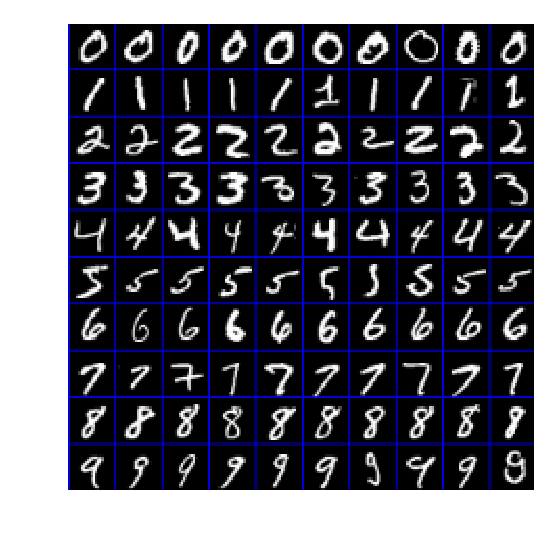
\includegraphics[width=4cm]{figures/mnist_original}  
   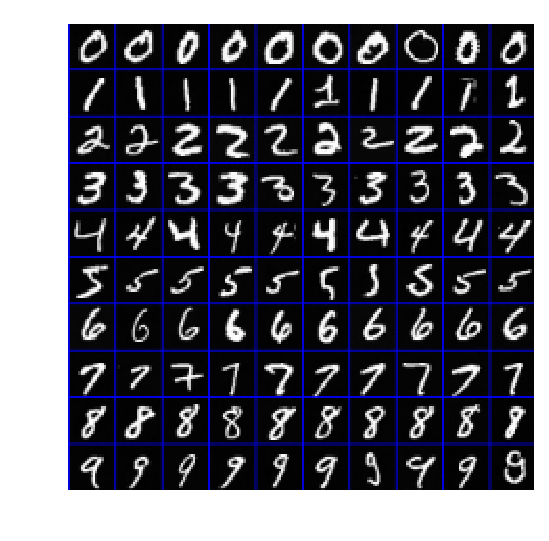
\includegraphics[width=4cm]{figures/mnist_reconstruction} 
   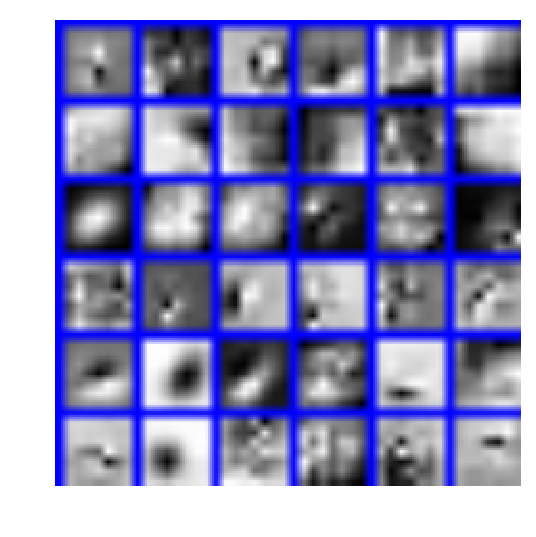
\includegraphics[width=4cm]{figures/mnist_dictionary}
   \caption{\small{Performance on the MNIST dataset. (Left) Training data. (Middle) Reconstructed digits. (Right) Learned dictioinaries. }} \label{fig:mnist}
\end{figure}

The root mean squared error (RMSE) is shown in Figure \ref{fig:mse}. After 500 iterations, we can achieve an RMSE of 0.23. As can be seen in Figure \ref{fig:mnist}, the convolutional factor analysis can reconstruct the digits almost perfectly. However, using a model like PCA can make the reconstructed images blurry.

\subsection{Caltech 101 Face Examples}

We next consider the Caltech 101 dataset \footnote{http://www.vision.caltech.edu/ImageDatasets/Caltech101/}, in which we perform analysis on 128 face images, and each image is resized to $32 \times 32$. The dictionary $\dv_k$ size is also set to $7 \times 7$.

\begin{figure}[h]
   \centering
   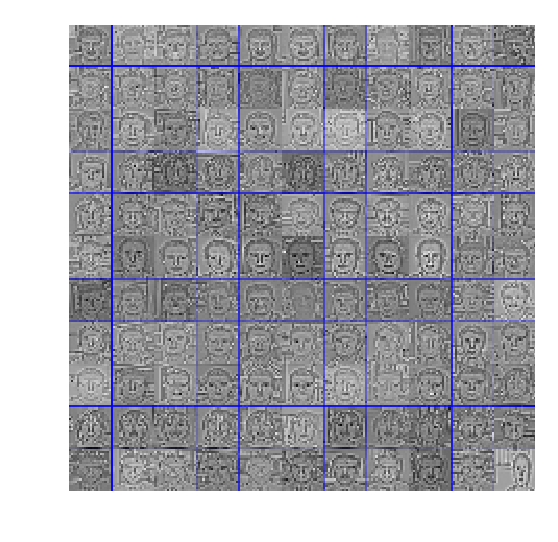
\includegraphics[width=4cm]{figures/face_original}  
   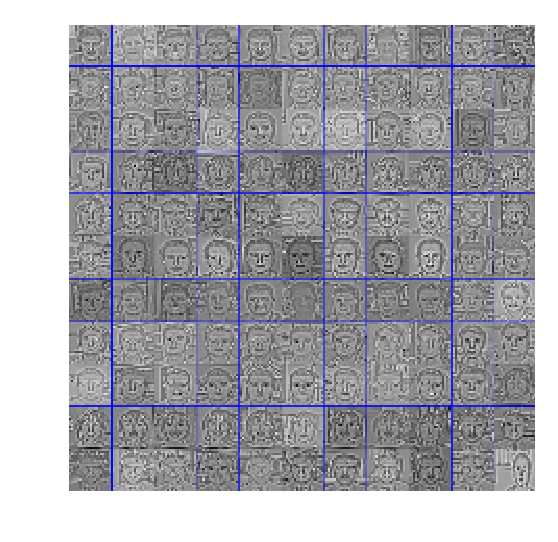
\includegraphics[width=4cm]{figures/face_reconstruction} 
   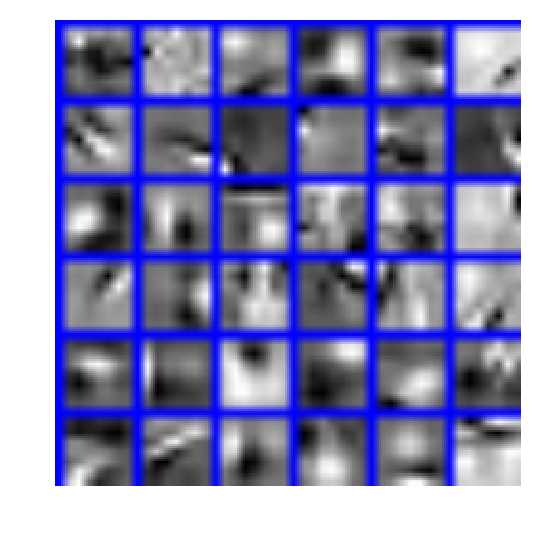
\includegraphics[width=4cm]{figures/face_dictionary}
   \caption{\small{Performance on the Caltech 101 face dataset. (Left) Training data. (Middle) Reconstructed digits. (Right) Learned dictioinaries. }} \label{fig:face}
\end{figure}

The root mean squared error (RMSE) is shown in Figure \ref{fig:mse}. After 500 iterations, we can achieve an RMSE of 4.40. As can be seen in Figure \ref{fig:face}, the faces are almost perfectly reconstructed.

Now, we compare our implemented convolutional factor analysis (CFA) algorithm with simple PCA. For fair comparison, we select the first $K=36$ principal components of PCA to recover the input images. The results are summarized in Table \ref{tab:table}. As can be seen, the performance of CFA is much better compared with simple PCA. 
%
\begin{table}[h]
\centering
\begin{tabular}{|c|c|c|}
\hline
\hline
Dataset & CFA & PCA  \\
\hline
MNIST & 0.23 & 2.47 \\
\hline
Caltech 101 Face & 4.40 & 23.86 \\
\hline
\end{tabular}
\caption{Comparison between CFA and PCA} \label{tab:table}
\end{table}

\section{Conclusion}
%
In this course project, we developed the convolutional factor-analysis model and implemented the Gibbs sampling algorithm for posterior inference. Experimental results on MNIST and Caltech 101 Face datasets show that the CFA model can achieve good performance.  

We tried to implement the deep extension of the CFA model, but failed to achieve good performances. This can be an interesting future work.

\bibliography{project}

\end{document}
